\section{Introduction}
\label{sec:ftag-intro}

For the physics program of the ATLAS experiment at the Large Hadron Collider (LHC), the identification of jets initiated by $b$-quarks, or $b$-tagging, is a fundamental tool. 
Ensuring its optimal performance is particularly important for the study of the Higgs boson and the top quark \cite{HIGG-2018-04, HIGG-2018-13}, as well as many exotic extensions of the Standard Model with resonances preferentially decaying to heavy quarks \cite{ATLASdijetres}. 


\begin{figure}[htbp]
  \centering
  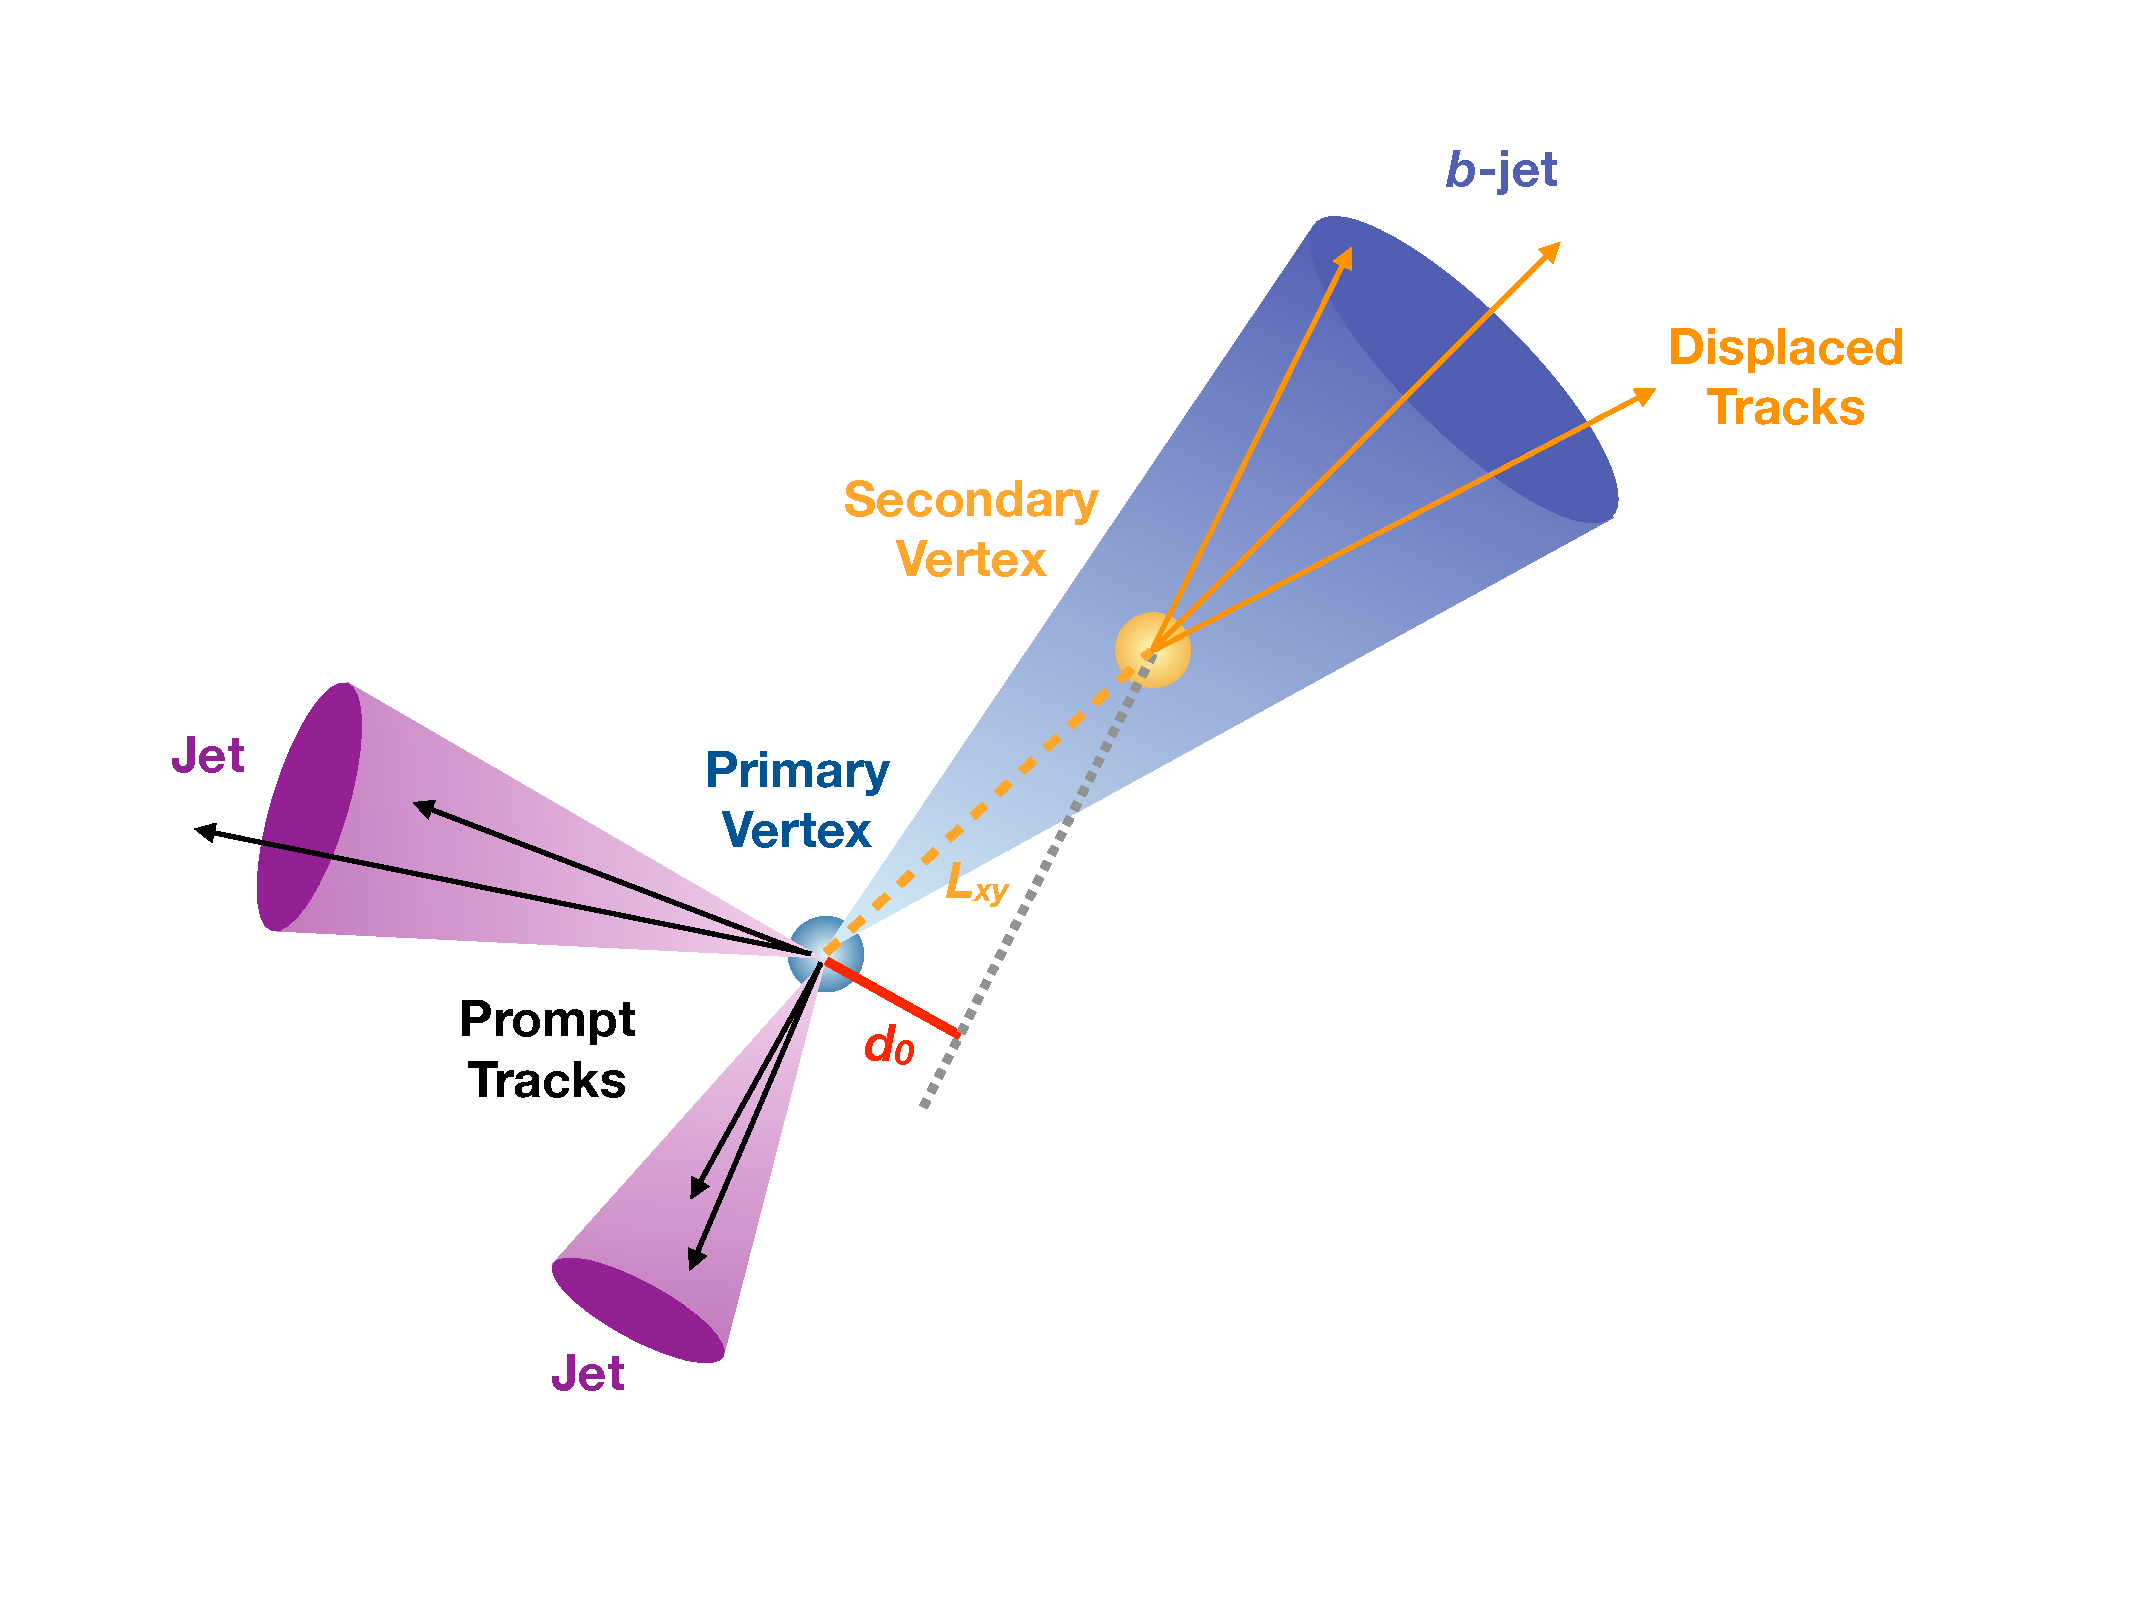
\includegraphics[width=0.9\textwidth]{figures/ftag/b-trig-paper/fig_01}
  \caption{Schematic illustration for the characteristic ``long'' lifetime of a \Pqb-hadron \cite{b-trig-paper}. }
  \label{fig:b-jet-graphic}
\end{figure}

The characteristically long lifetime of hadrons containing $b$-quarks ($b$-hadrons) of the order of 1.5 ps \cite{PDG} leads to two classes of $b$-tagging algorithms: \textit{vertexing} based algorithms which explicitly reconstruct a production point, or vertex, of the $b$-hadron decay displaced from the primary interaction point, and track based algorithms which exploit the displacement of the reconstructed charged particles trajectories (tracks) produced in $b$-hadron decays from the primary interaction point.

%We then use a NN to combine information from these low-level algorithms into a high level tagger and we refer to these collection of algorithm to solve the classification problem of identifying jets containing a $b$-quark as $b$-tagging.


\begin{figure}[htbp]
  \centering
  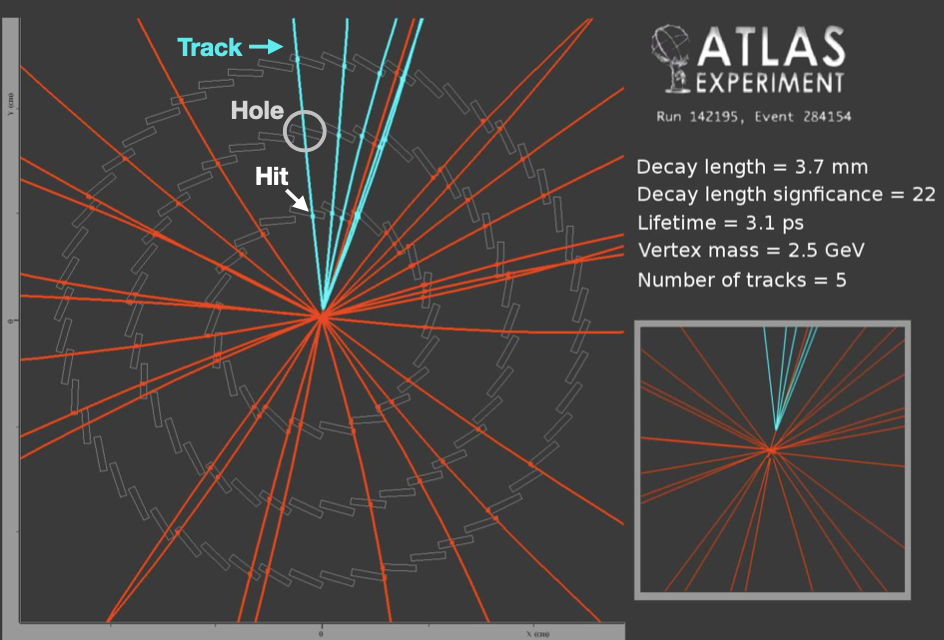
\includegraphics[width=0.9\textwidth]{figures/ftag/b-decay-evt-display-annotated}
  \caption{Illustration of what a b-decay looks like in the ATLAS detector. 
  The cyan colored lines illustrate the tracks from the \Pqb-hadron decay, and in the inset figure you can see the displacement of these tracks from the primary vertex. 
  Only three pixel layers are shown as this is a Run~1 event, and the IBL was not yet installed. \hl{Need to revise older notes to find where this event display came from (or ask Su Dong)}. }
  \label{fig:b-jet-graphic}
\end{figure}

ATLAS employs several IP-based algorithms which are later combined with vertexing algorithms to produce a "high-level" tagger for general use.


\begin{figure}[htbp]
  \centering
  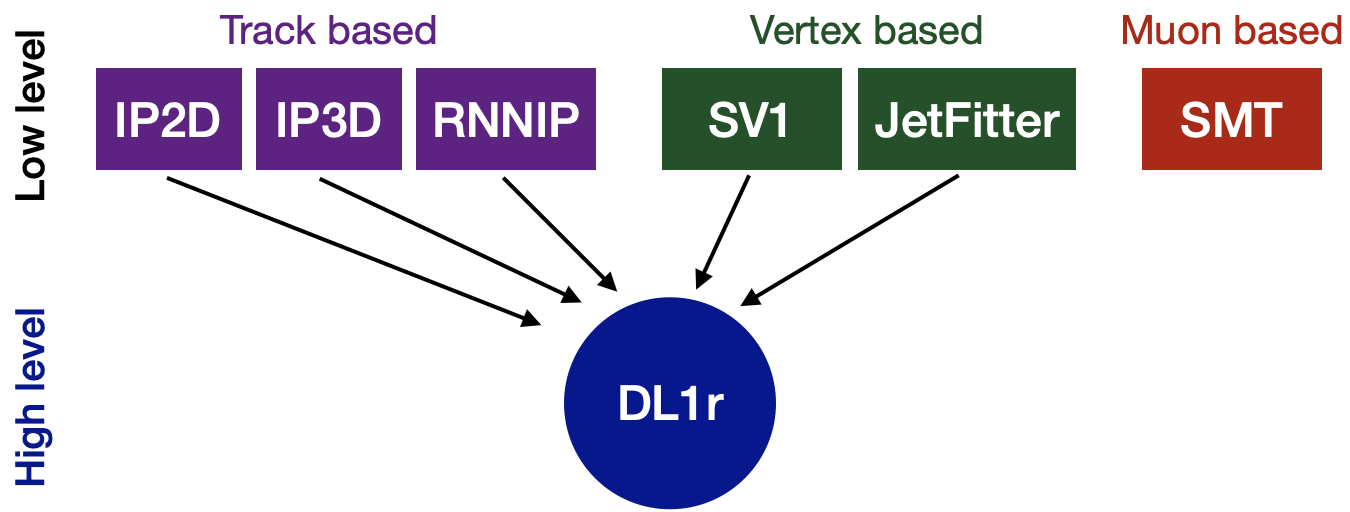
\includegraphics[width=0.9\textwidth]{figures/ftag/ATLAS-taggers}
  \caption{Types of \Pqb-taggers used on ATLAS}
  \label{fig:ATLAS-taggers}
\end{figure}

This chapter is organized as follows: Section \ref{sec:datasets} describes the datasets and selections used to train and evaluate the algorithms, while section \ref{sec:alg} details impact parameter based taggers, the Deep Sets algorithm and our specific implementation. Section \ref{sec:results} shows investigations of what the network has learned, results for the timing metrics, discussion on calibrating the algorithm, and the optimization studies conducted. Finally, section \ref{sec:conclusion} summarizes the conclusions.
